\chapter{新闻事件的主题演化分析}
第二章,我们介绍了文本分析的常用方法,以及它们在具体场景的应用。然而这些方法并没有考虑文本的产生的时间,在建模时简单认为文本之间是可交换的。显然这样的处理方式不够充分,因为在现实情况中,大部分文本(如,新闻报道,学术文章)都具有时间属性。对同一事物或事件的叙述,随着时间的推移一定会产生变化,而这些变化之间的差异又必然会存在一定的依赖关系。本章,我们将重点研究新闻语料的特点,并基于此提出一套有效的方法来跟踪新闻事件的主题演化过程。

\begin{assumption}
\label{hyp:newsdistribution}
对于同一个新闻事件的报道往往呈现出多个阶段,且每个阶段内报道的文章都是针对同一个方面,文章有很高的相似性。
\end{assumption}

\begin{assumption}
\label{hyp:coherence}
如果语料库中文本之间的一致性越高,那么用主题模型分析,挖掘出的信息也就越丰富。
\end{assumption}

\section{新闻事件的时序分析}
已有的动态主题模型,如:TOT模型\cite{wang2006topics}将文档的时间戳作为一个标签,并且认为文档的生成过程同时受主题~词分布和文档的时间戳两个因素的影响;cDTM模型\cite{wang2008continuous}用布朗运动来模拟不同时间段内主题之间的演化关系,该模型相比DTM模型\cite{Blei:2006}不需要将时间序列离散化,可以称之为连续的动态主题模型。这些模型虽然各有不同,但追根究底都是通过一个模型来模拟主题随时间推移,是如何从前一个阶段演化到后一个阶段。然而对于一个特定集合的文档来说,集合中所有文档都是关于同一个主题,并且在每一个时间段内都可能出现新的子主题,用已有的这些模型很难捕捉新产生的模型,因而就不能去挖掘文档集合中更深层次的子主题信息。后面,我们通过对新闻报道本身的时序分布信息进行分析,并探索如何将该信息与主题模型结合来追踪某个事件的主题演化。
\subsection{新闻报道的时序分布}
当某一重大新闻事件$E_1$爆发时,通常在较短的时间内,各大媒体都会争相报道,此时关于此事件的报道数量会迅速达到一个峰值$P_1$。随着时间的推移该事件开始慢慢降温,或发生了其他更具吸引力的事件$E_2$,关于事件$E_1$的报道数量也会回落到一个较小的范围。然而,对于重要的新闻事件,随着时间的发展,不时会有新的信息被披露,每一次信息的披露都会让该事件重新获得上头条的机会,那么新闻的报道数量也就会重新攀升至一个新的峰值$P_2$。如此往复,重大新闻事件往往会经历几个阶段。

如果我们将事件$E_1$每次报道数量达到峰值前后一段时间一起作为一个阶段,虽然在这个阶段内新闻的报道数量会非常多,但是实际上大部分的报道内容都非常的相似,因为各家媒体获得信息都差不多。然后,不同的阶段之间,报道的内容会有较大的不同。我们从英国卫报(The Guardian) \footnote{http://www.theguardian.com/} 上分别抓取了以 Edward Snowden 和 Obamacare 为关键词的新闻报道,图 \ref{fig:temporal-dist}表示了它们的时序分布情况,X轴表示时间(单位:天),Y轴表示新闻的报道数量(单位:篇)。正如我们的猜想,新闻报道的实际时序分布的确包含了多个波峰和波谷。
% BEGIN == 新闻报道的时序分布图
\begin{figure}[htb]
	\centering
	\subfloat[Edward Snowden]{
		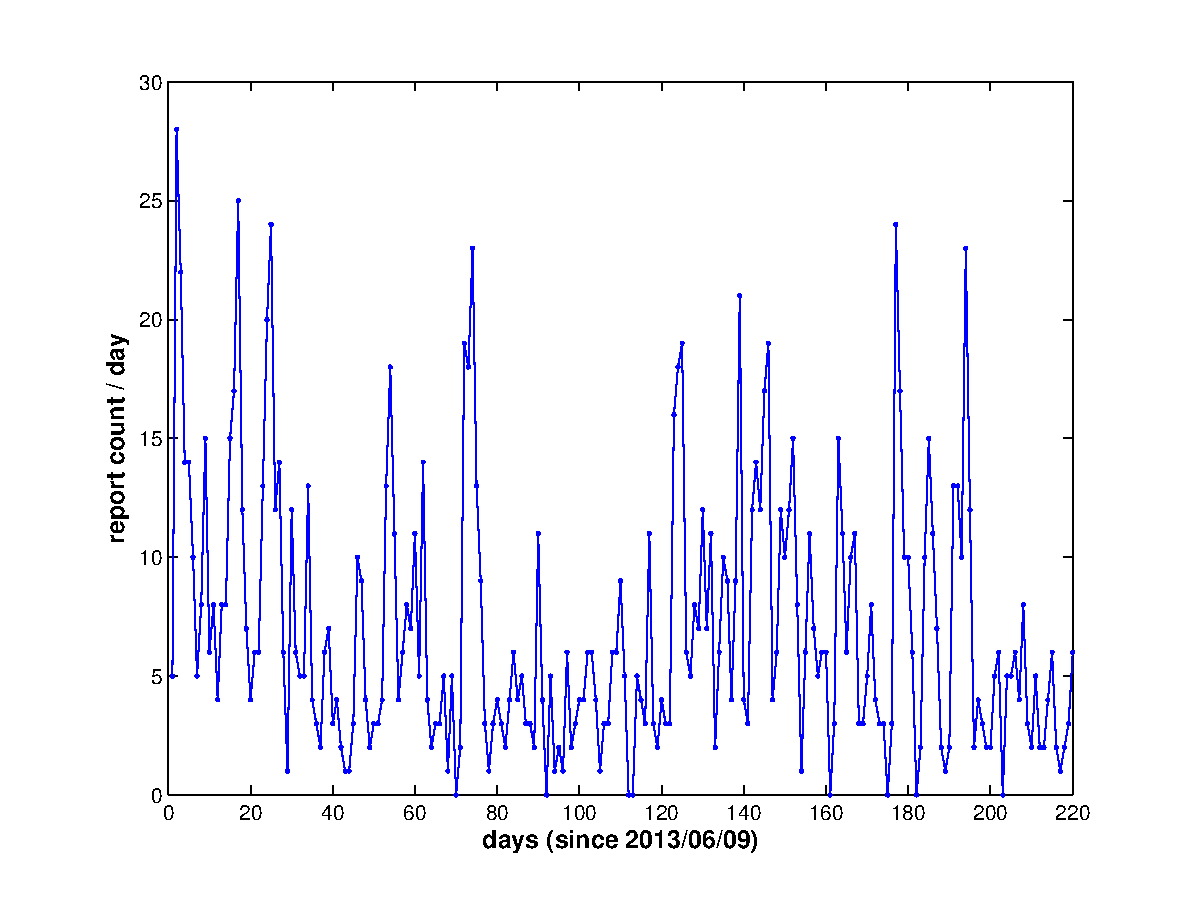
\includegraphics[width=0.5\textwidth]{guardian_snowden}
		\label{fig:temporal-dist:snowden}}
	\subfloat[Obamacare]{
		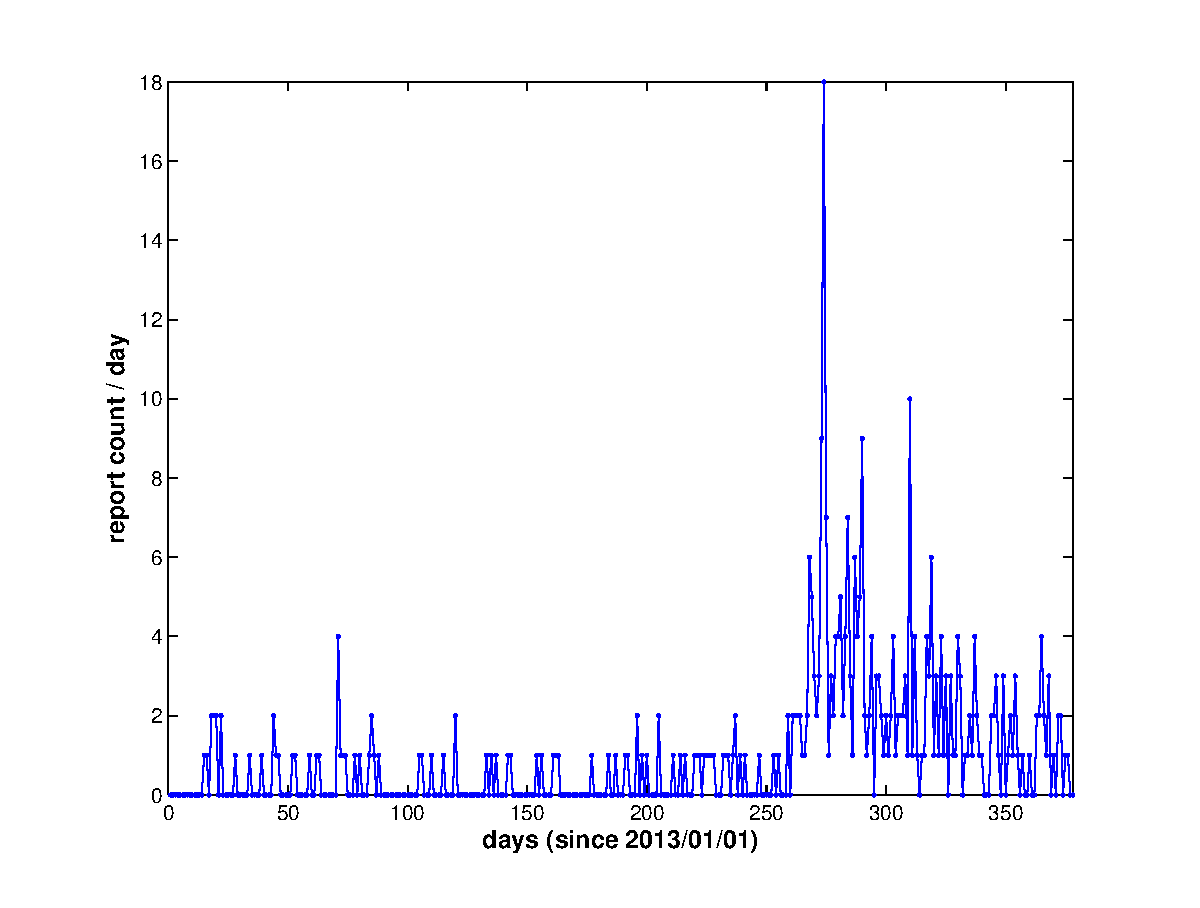
\includegraphics[width=0.5\textwidth]{guardian_obamacare}
		\label{fig:temporal-dist:obamacare}}
	\caption{新闻报道数量的时序分布图}
	\label{fig:temporal-dist}
\end{figure}
% END == 新闻报道的时序分布图

\subsection{新闻语料的时序划分}
\label{sec:ada-kmeans}
DTM \cite{Blei:2006}是由David Blei等人提出的动态主题模型,该模型将语料库均匀(如按年,月,日等)划分为多个子集,由此获得的每个子集时间跨度都相同。然而,根据上一小节的分析可以知道,均匀划分语料库的方法显然有许多不妥之处。首先,各个子集的文本数量上可能会有很大的差异,有的子集文本数量非常多,有点非常少;其次,均匀划分时前后时间段的分割点,可能恰好落在 图 \ref{fig:temporal-dist} 所示的波峰位置,这样就把一堆一致性非常高的文本划分到了两个阶段。

基于上面的分析,我们可以得到一个合理的划分语料库所需满足的几个条件:
\begin{inparaenum}[\itshape 1 \upshape)]
\item 每个时间段内的文本具有较高的一致性,它们可能都是报道事件的同一个方面或同一个进展;
\item 尽量保障每个时间段的文档数量不要太少。
\end{inparaenum}
从 图 \ref{fig:temporal-dist} 来看的话,符合上面条件的好的分割点应该是落在波谷附近。

为了实现语料库的自动划分,我们设计了一个自适应的聚类算法Adaptive K-Means Algorithm. 该算法是基于K-Means \cite{kanungo2002efficient} 改进而来,弥补了K-Means需要手动设置聚类数的不足。该算法是一个迭代算法,每一次迭代将聚类数目加1,并且计算本次迭代结束后,聚类中所有点离其中心点的加权平均距离(Weighted Mean Distance),该距离公式定义如下:
\begin{equation}
\label{eq:wmd}
Weighted\;Mean\;Distance=\frac{\sum_{i=1}^{n}{mean\;distance\;of\;cluster\;i}}{n}
\end{equation}
每次迭代结束后,将当前的加权平均距离$WMD_i$与前一次迭代获得的加权平均距离$WMD_{i-1}$相减,若加权平均距离的减少量达到预设的阀值,则迭代结束,此时的聚类数目便是最佳的聚类数。公式 (\ref{eq:wmd}) 中的距离使用的是二维空间中的欧式距离, 算法的伪代码描述见 Algorithm \ref{algo:ada-kmeans}。

% BEGIN == 自适应聚类算法 伪代码
\begin{algorithm}
  \DontPrintSemicolon
  \KwData{$X$: news count of each day; $max\_k$: the maximum value of K; $t$: threshold value}
  \KwResult{$count$: article count of each episode; $dists$: weighted mean distance array; $K$: the best count of cluster}
  \BlankLine
  $Y \longleftarrow$ remove $zero$ points from $X$\;
  \For{$i \leftarrow 1$ \KwTo $max\_k$}{
    $[count, sumd]=kmeans(Y, i)$;\;
    \tcp*[r]{$count$: point count of each cluster}
    \tcp*[r]{$sumd$: sum distance of each cluster}
    $means \leftarrow calcMeanDistance(count, sumd)$;\;
    \tcp*[r]{$means$: mean distances of all clusters}
    $dists[i] \leftarrow calcWeightedMeanDistance(means)$;\; 
    \If{$i > 1$} {
      \If{$dists[i]-dists[i-1] < t$}{
        $K \leftarrow (i-1)$; break;
      }
    }
  }
  \If{$K = 0$} {$K \leftarrow max\_k$;\;}
  \caption{Adaptive K-Means Algorithm}
  \label{algo:ada-kmeans}
\end{algorithm}
% END == 自适应聚类算法 伪代码

\subsubsection{异常点修正}
通过以上算法获得的划分会出现一些奇异点会被划分到相邻的聚类中,为了保证聚类 $Cluster_i$ 内的所有点在时间轴上均小于 $Cluster_{i+1}$ 并大于 $Cluster_{i-1}$ 内的点,我们需要对通过以上算法获得的结果进行一些修正。修正的方法如Algorithm \ref{algo:cluster_correction}所示:\par
% BEGIN == 自适应聚类算法 伪代码
\begin{algorithm}
  \DontPrintSemicolon
  \BlankLine
  $sortClusterByTime(clusters)$\;
  \For{each cluster $c_i$ in all clusters}{
    \For{each point $p_j$ in $c_i$}{
      \If{$x_{p_j}$ < $min(x_{c_i})$ or $x_{p_j}$ > $max(x_{c_i})$}{
        $reassignClusterLabel(p_j)$\;
      }
    }
  }
  \caption{Cluster Correction Algorithm}
  \label{algo:cluster_correction}
\end{algorithm}
上面算法中的$reassignClusterLabel(p_j)$是根据点$p_j$的X轴坐标值进行分配,只需要将$x_{p_j}$与各个聚类的x轴上限值和下限值做比较,若在上下限值中间,即可将点$p_j$归为该类。

\subsubsection{其它划分方法分析}
Adaptive K-Means Algorithm 简单高效,而且通过 \ref{sec:ada-kmeans-result} 小节的实验结果可以看出,划分出来的结果也很好的满足了上述的划分要求。然而,我们并没有在一开始就想到利用聚类进行语料库的划分,而是在尝试了多种方法之后才发现了这一比较巧妙的方法。我们尝试了以下几种方法,但均未能获得较好的实验结果:
\begin{inparaenum}[\itshape a \upshape)]
\item 首先通过多项式拟合,获得一个符合报道分布趋势的多项式曲线,这样一来,多项式曲线的极小值点便是接近峰谷位置的点,只需求出曲线的所有极小值点,便得到了语料划分的临界点。但是通过实验我们发现,由于一些特殊点的影响,即使是十几次方的曲线仍然不能很好的符合报道的真实分布情况。
\item 我们还尝试将报道的时序分布看成是波形图,使用卡尔曼滤波和小波分析的方法去分析,结果同样不尽如人意。
\end{inparaenum}

\section{结合时序信息的主题模型}
本章节主要介绍我们如何将新闻文档的时序分布信息结合到主题模型,并通过这个结合的模型去分析时序文本的主题演化,得到主题演化图。最后,我们我们会分析为什么结合时序分布信息后能有效的增强主题模型的效果。
\subsection{基本概念}
\label{sec:concepts}
首先,我们将给出一些名词定义,它们将会在下文中频繁出现。

阶段(Stage)一个阶段就是一个时间区间,在一个阶段内的新闻报道往往有很强的一致性,它们很可能报道的都是事件的同一个方面。

主要主题(Main Topic)对于同一个事件,它从 $stage_{i-1}$ 发展到 $stage_i$  的过程中,报道围绕的焦点都是事件本身,我们将这个贯穿整个事件发展周期的焦点作为事件的主要主题,事件的主要主题随着时间推移变化很小。

辅助主题(Auxiliary Topic)同时,在事件发展的各个阶段,更能反映这段时间内新动向和进展的往往不是主要主题,而是除它以外的其它主题,我们将其称为辅助主题。辅助主题随时间推移变化较为显著,而正是辅助主题的变化反应了事件的演化。

\subsection{整体框架}
\label{sec:framework}
我们的分析框架是基于LDA(Latent Dirichlet Allocation)\cite{Blei:2003}模型。LDA 是一个生成式模型,它的基本思想是:将每个文档看成是一个词的袋子,每个词都是通过文档的一个或多个主题确定的。形式化表示,可以将文档表示成一个主题的多项式分布,同时每一个主题又可以看成是词语的多项式分布。对于模型的参数评估我们采用 Collapsed Gibbs Sampling \cite{griffiths2004finding, heinrich2005parameter}。 LDA 模型假设所有文档都是可交换的,显然对于新闻,邮件,学术文章等时序文本并不满足可交换性。对于这类时序文本的分析,\ref{intro-dtm} 小节介绍了经典的 DTM 模型,然而正如我们在 \ref{sec:ada-kmeans} 小节中的分析,它也有自己的局限性。因此,本小节我们将提出我们的自己的一个分析方法。首先,我们将利用 \ref{sec:ada-kmeans} 小节中提出的方法对语料库进行划分,将一个大的语料库划分成时间区间,文章数目不等的多个子语料库,然后在对各个子语料库中分别利用 LDA 模型进行主题抽取,最后分析各个子语料库间的关联性,并画出主题演化图。图 \ref{system-overview} 详细描述了框架的各个步骤:
\begin{enumerate}[(1)]
\item 语料集获取。在后面的实验分析中,我们采用的语料库是自己编写爬虫程序从新闻网站  The Guardian 上根据不同的关键词爬取下来的,然而直接爬取下来的是完整的html页面,我们需要从html代码中解析出文章的正文内容。在进行html解析和正文获取时,我们借鉴了稍后阅读服务 Readability \footnote{https://readability.com/} 的解析算法,并在此基础上开发了一套html解析程序。
\item 语料库划分。语料库划分的目的是将一个大的语料库划分成多个子语料库,划分的时候既要保证将一致性高的文档划分在同一个子集中,又要保证时序上的一致性,相邻子集在时间上时连续的承接关系,并且子集中的文章也必须发生在该时间段内。详细的文档划分方法可以参见 \ref{sec:ada-kmeans} 小节,划分结果可以参见 \ref{sec:ada-kmeans-result} 小节。
\item 文档预处理。文档预处理是指将文档表示成词袋的过程,在我们的分析中,每篇文章预处理后的结果是,由各个词以及它在文章中出现的频次组成的序列,并且需要将语料库中产生的所有词进行统一编号。文档预处理中用到的方法,包括了:分词,词性标注(只保留名次,专有名词,动词和形容词),去停用词,去低频词,词形还原。实验中,我们使用开源工具包 Stanford Parser \footnote{http://nlp.stanford.edu/software/lex-parser.shtml}进行分词,词性标注和还原。
\item 模型构建与参数学习。我们在每个子语料库上构建 LDA 模型,并通过 Collapsed Gibbs Sampling \cite{griffiths2004finding, heinrich2005parameter} 方法进行参数学习,从而得到每个子语料库上的主题分布。
\item 主题关联分析。在获得每个子语料库的主题分布后,我们需要计算相邻子集之间所有主题两两之间的相似度,从而发现语料库的主要主题,\ref{sec:similairty-calc} 小节将详细介绍如何度量主题的相似度。
\item 事件演化图绘制。最后,我们需要将事件的主题演化进行可视化展示,我们采用 Graphviz\footnote{http://www.graphviz.org}工具包,通过Python语言实现了一个能自动绘制演化图的程序。在演化图中,对于每个时间段,我们仅取概率最大的前三个主题,并且用有向线段串接主要主题。具体的结果参见 \ref{sec:evolution-map} 小节。
\end{enumerate}
% BEGIN == 新闻报道的时序分布图
\begin{figure}[!htb]
    \includegraphics[width=\textwidth]{system_overview}
    \caption{结合时序信息的主题模型分析框架}
    \label{system-overview}
\end{figure}
% END == 新闻报道的时序分布图

\subsection{主题相似度计算}
\label{sec:similairty-calc}
正如 \ref{sec:concepts} 小节所定义的,主主题是贯穿这个事件的主线,在两个相邻的时间段内,主主题之间的相似度要高于其它所有两两主题间的相似度。为了发现跟踪事件的发展,我们首先要从每个时间段中找出衔接前后时间段的主主题。为此,我们就需要计算相邻时间段内所有主题之间的两两相似度,例如:在 $stage_i$ 中共有10个主题分别为$\{t_i^i, t_i^2, ..., t_i^{10}\}$,在 $stage_{i+1}$ 中的10个主题分别为 $\{t_{i+1}^i, t_{i+1}^2, ..., t_{i+1}^{10}\}$, 我们需要进行相似度计算的组合就有100对。主题模型中主题是用词的多项式分布表示的,通常我们可以通过 Kullback-Leibler divergence(也被称为 relative entropy)来计算概率分布的相似性。对于离散的概率分布 $P$ 和 $Q$ 而言,它们的 KL divergence 可以定义如下:
\begin{equation}
D_{KL} \left ( P||Q \right ) = \sum_{i}ln\left ( \frac{P(i)}{Q(i)} \right ) P(i)
\end{equation}
然而,KL divergence 并不是一个最佳的距离测度,因为它是非对称的。Jensen-Shannon distance 是 KL divergence 的平滑且对称的扩展版本,它的定义如下:
\begin{equation}
D_{JS} \left ( P||Q \right ) = \frac{1}{2} D_{KL} \left ( P||M \right ) + \frac{1}{2} D_{KL} \left ( Q||M \right )
\end{equation}
其中,$M = \frac{1}{2}(P+Q)$。

\subsection{文本一致性及其度量}
文本一致性(Coherence) 度量的是文本之间主题的相似性。两个文本的一致性越高,表示这两篇文本的描述的内容越相似。从直觉角度出发,通常如果有一堆文本,如果这堆文本相互之间的一致性越高,那么用主题模型对文档集合进行建模时,能够挖掘的信息也就越丰富。以图 \ref{fig:temporal-dist} 中我们抓取的两个事件的新闻报道为例:
\begin{inparaenum}[\itshape 1 \upshape)]
\item 我们将所有的报道全部作为一个集合进行主题挖掘;
\item 我们将各自事件的报道分开作为两个集合,分别进行主题挖掘。
\end{inparaenum}那么很显然方法二,所能挖掘出来的信息会更具体,我们能从方法二获得的事件的信息更多。

换言之,如果我们在使用主题模型进行文本分析时,如果在同一个时间区间内的文本之间一致性越高,那么结果就会更显著,对事件的理解也会更深入。通常我们可以利用方差来度量数据的一致性,但是它却不能很好的体现文本主题的一致性,因此我们通过主题覆盖率(n Topic Coverage Rate, $TCR_n$)来间接的度量,定义如下:
\begin{equation}
\label{eq:tcr}
TCR_n = \frac{\left \| articles\;\;belong\;to\;these\;n\;topics \right \|}{\left \| all\;articles \right \|} * 100\%
\end{equation}
在公式 (\ref{eq:tcr}) 中,$\left \| \cdot \right \|$表示集合中元素的数量,$TCR_n$度量最相关的前n个主题对文本的覆盖率。从公式 (\ref{eq:tcr}),我们可知,如果主题数$n$固定,那么$TCR_n$越大,文本之间的的一致性越高;同时,若$TCR_n$固定,那么主题数$n$越小,文本之间的一致性越高。


\section{实验结果和分析}
本小节中,我们通过实验结果来阐述以上提到的方法和度量指标。首先我们将通过两个语料库的数据来说明 \ref{algo:ada-kmeans} 的划分结果,它们分别是从英国卫报上爬下来的新闻数据,一个是根据关键词“Edward Snowden”,另一个是根据关键词“Obamacare”。接着我们重点分析“Edward Snowden”这个语料库,用我们 \ref{sec:framework} 小节中提出的分析框架进行分析,并得到事件发展的主题演化图。“Edward Snowden”这一语料库共包含文档1550篇,时间跨度从事件发生的2013年6月9号到2013年结束,整个语料库包含单词150万左右,通过预处理(每个单词至少出现5次),最终保留的的单词数为7732。
\subsection{语料库划分结果}
\label{sec:ada-kmeans-result}
% BEGIN == 语料库划分结果图
\begin{figure}[htb]
	\centering
	\subfloat[Edward Snowden]{
		\includegraphics[width=0.5\textwidth]{guardian_snowden_change}
		\label{fig:cluster-snowden-trend}
	}
	\subfloat[Edward Snowden]{
		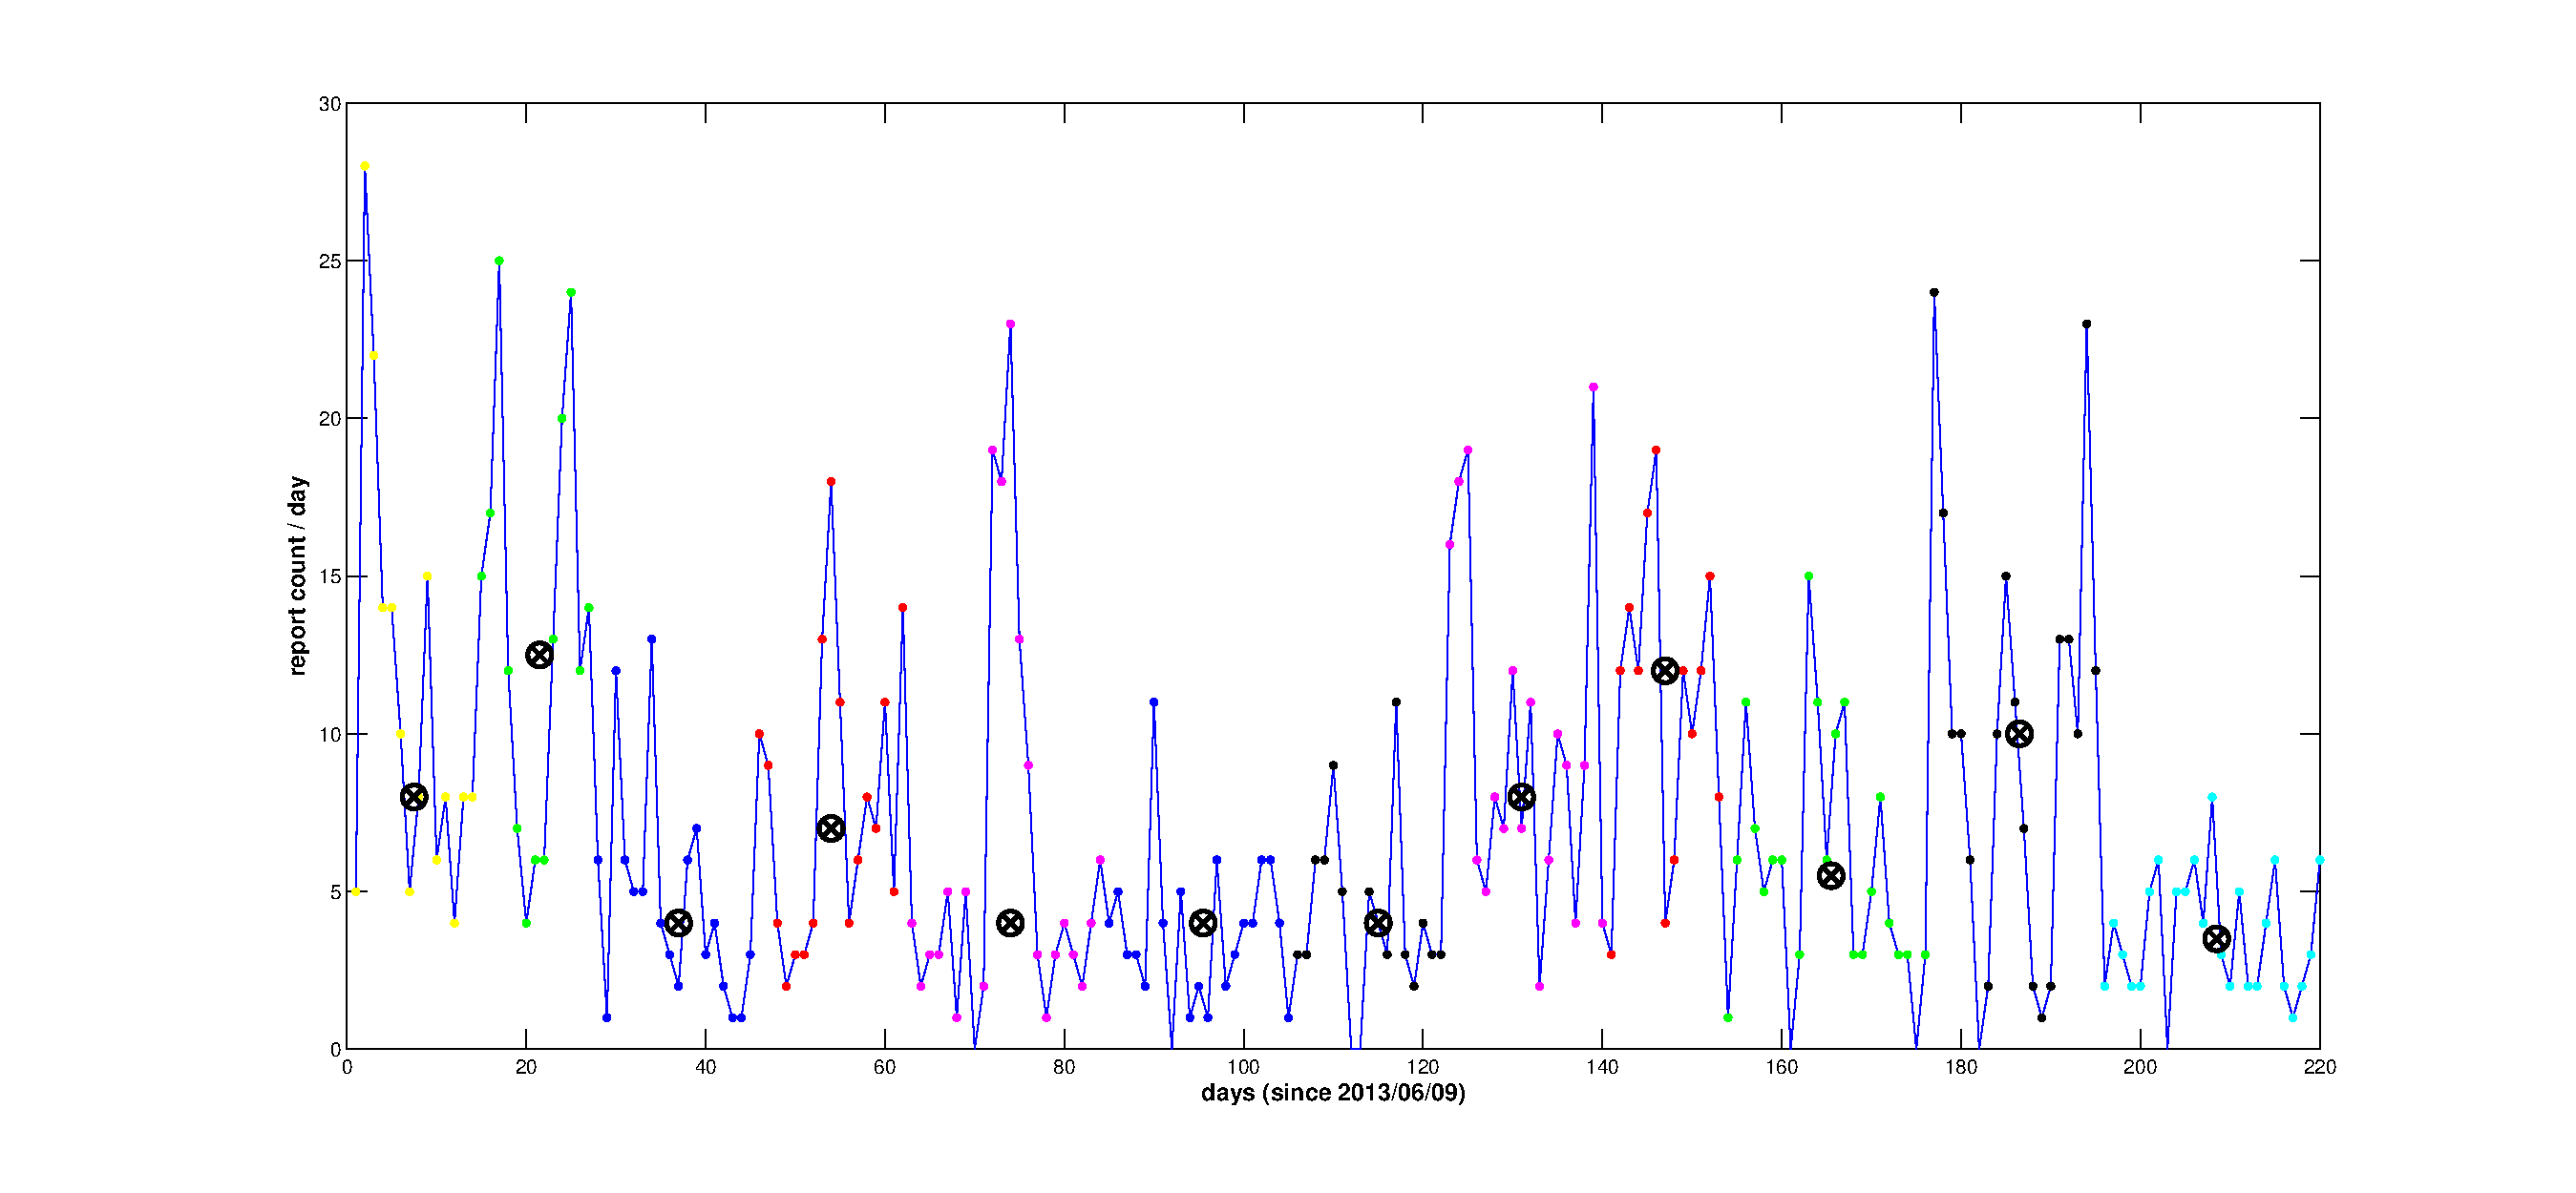
\includegraphics[width=0.5\textwidth]{guardian_snowden_cluster}
		\label{fig:cluster-snowden-result}
	}%需要换行,留一个空行

	\subfloat[Obamacare]{
		\includegraphics[width=0.5\textwidth]{guardian_obamacare_change}
		\label{fig:cluster-obamacare-trend}
	}
	\subfloat[Obamacare]{
		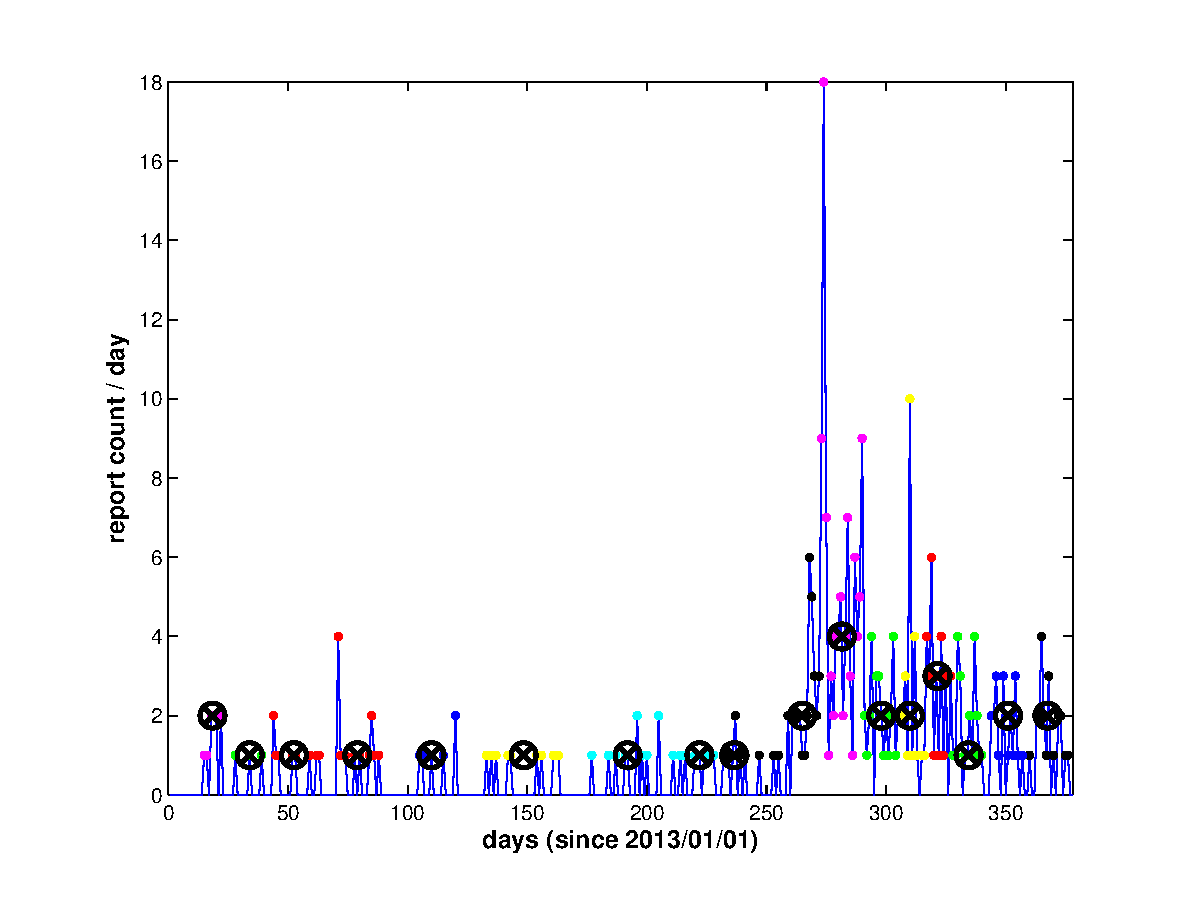
\includegraphics[width=0.5\textwidth]{guardian_obamacare_cluster}
		\label{fig:cluster-obamacare-result}
	}	
	\caption{聚类过程中平均加权距离的变化趋势以及最终的划分结果}
	\label{fig:cluster}
\end{figure}
% END == 语料库划分结果图
图 \ref{fig:cluster-snowden-trend}和\ref{fig:cluster-obamacare-trend} 中的$\otimes$ 表示最佳的时间段数目, 图 \ref{fig:cluster-snowden-result}和\ref{fig:cluster-obamacare-result} 中的 $\otimes$表示各个类的中心点,图 \ref{fig:cluster-snowden-result}和\ref{fig:cluster-obamacare-result}中的每种颜色分别代表一个聚类。
我们的语料库时间跨度相对较长,因此实验中我们设置的最大时间段数为20,另外通过反复的实验对比,我们将聚类加权平均距离的减小量阀值设为0.5。由于 adaptive k-means algorithm 是一个迭代算法,迭代的结束的条件是加权平均距离的减小量小于阀值,或者达到最大迭代次数。迭代结束时的时间段数目便是我们最终确定的阶段数目。图 \ref{fig:cluster} 分别展示了两个语料库的最终划分结果,以及迭代过程中加权平均距离的变化趋势。

\subsection{主题演化图分析}
\label{sec:evolution-map}
考虑到语料库是针对某一个具体的新闻事件,因此主题的数并不会太多,在绘制主题演化图时我们仅选取了概率最大的前三个主题,其中一个为主主题,两个为辅助主题。图 \ref{fig:evolution-our}是通过本文提出的方法获得的主题演化图;图 \ref{fig:evolution-even} 与 图 \ref{fig:evolution-our} 的不同之处在于语料库的划分方式不同, 图 \ref{fig:evolution-even}  是通过时间均匀划分得到的子语料库;图 \ref{fig:evolution-dtm} 是通过 DTM 模型得到的主题演化图。三种方法所划分的时间段数目都一样 \footnote{每个时间段内标注的日期表示该阶段的起始日期,同时也是前一个阶段的结束日期}。

其中 图 \ref{fig:evolution-our} 和 图 \ref{fig:evolution-even}中的有向箭头连接的是整个语料的的主主题。对比这两张演化图,我们可以很明显的发现,采用本文提出的语料库划分算法,最终的得到的主主题在不同时间段内都能很好的保持连续性,它始终是相邻两个时间段内相似度最高的两个主题。而采用均匀划分语料库的方法得到的主题演化图,主主题在第4和第5个时间段内发生了变化,同样在第5和第6个时间段内再一次发生了变化,这种主主题的不一致容易让读者误以为在这个时间点,语料库发生了变化,它们针对的可能并不是一个事件,不利于主题跟踪。

同样,通过对比 图 \ref{fig:evolution-our} 和 图 \ref{fig:evolution-dtm},我们可以发现 DTM 获得的主题演化图在各个时间段内主题几乎没有发生变化,例如时间段1-5内的主题1中概率最大的前10个单词是一模一样的,只不过出现的概率发生了细微变化,而其它几个主题的情况也差不多。对于这样的主题演化图,我们几乎不能从中得出时间随时间发展发生了怎样的变化。

% BEGIN == 采用本文方法获得的主题演化图
\begin{figure}[htb]
	\centering
	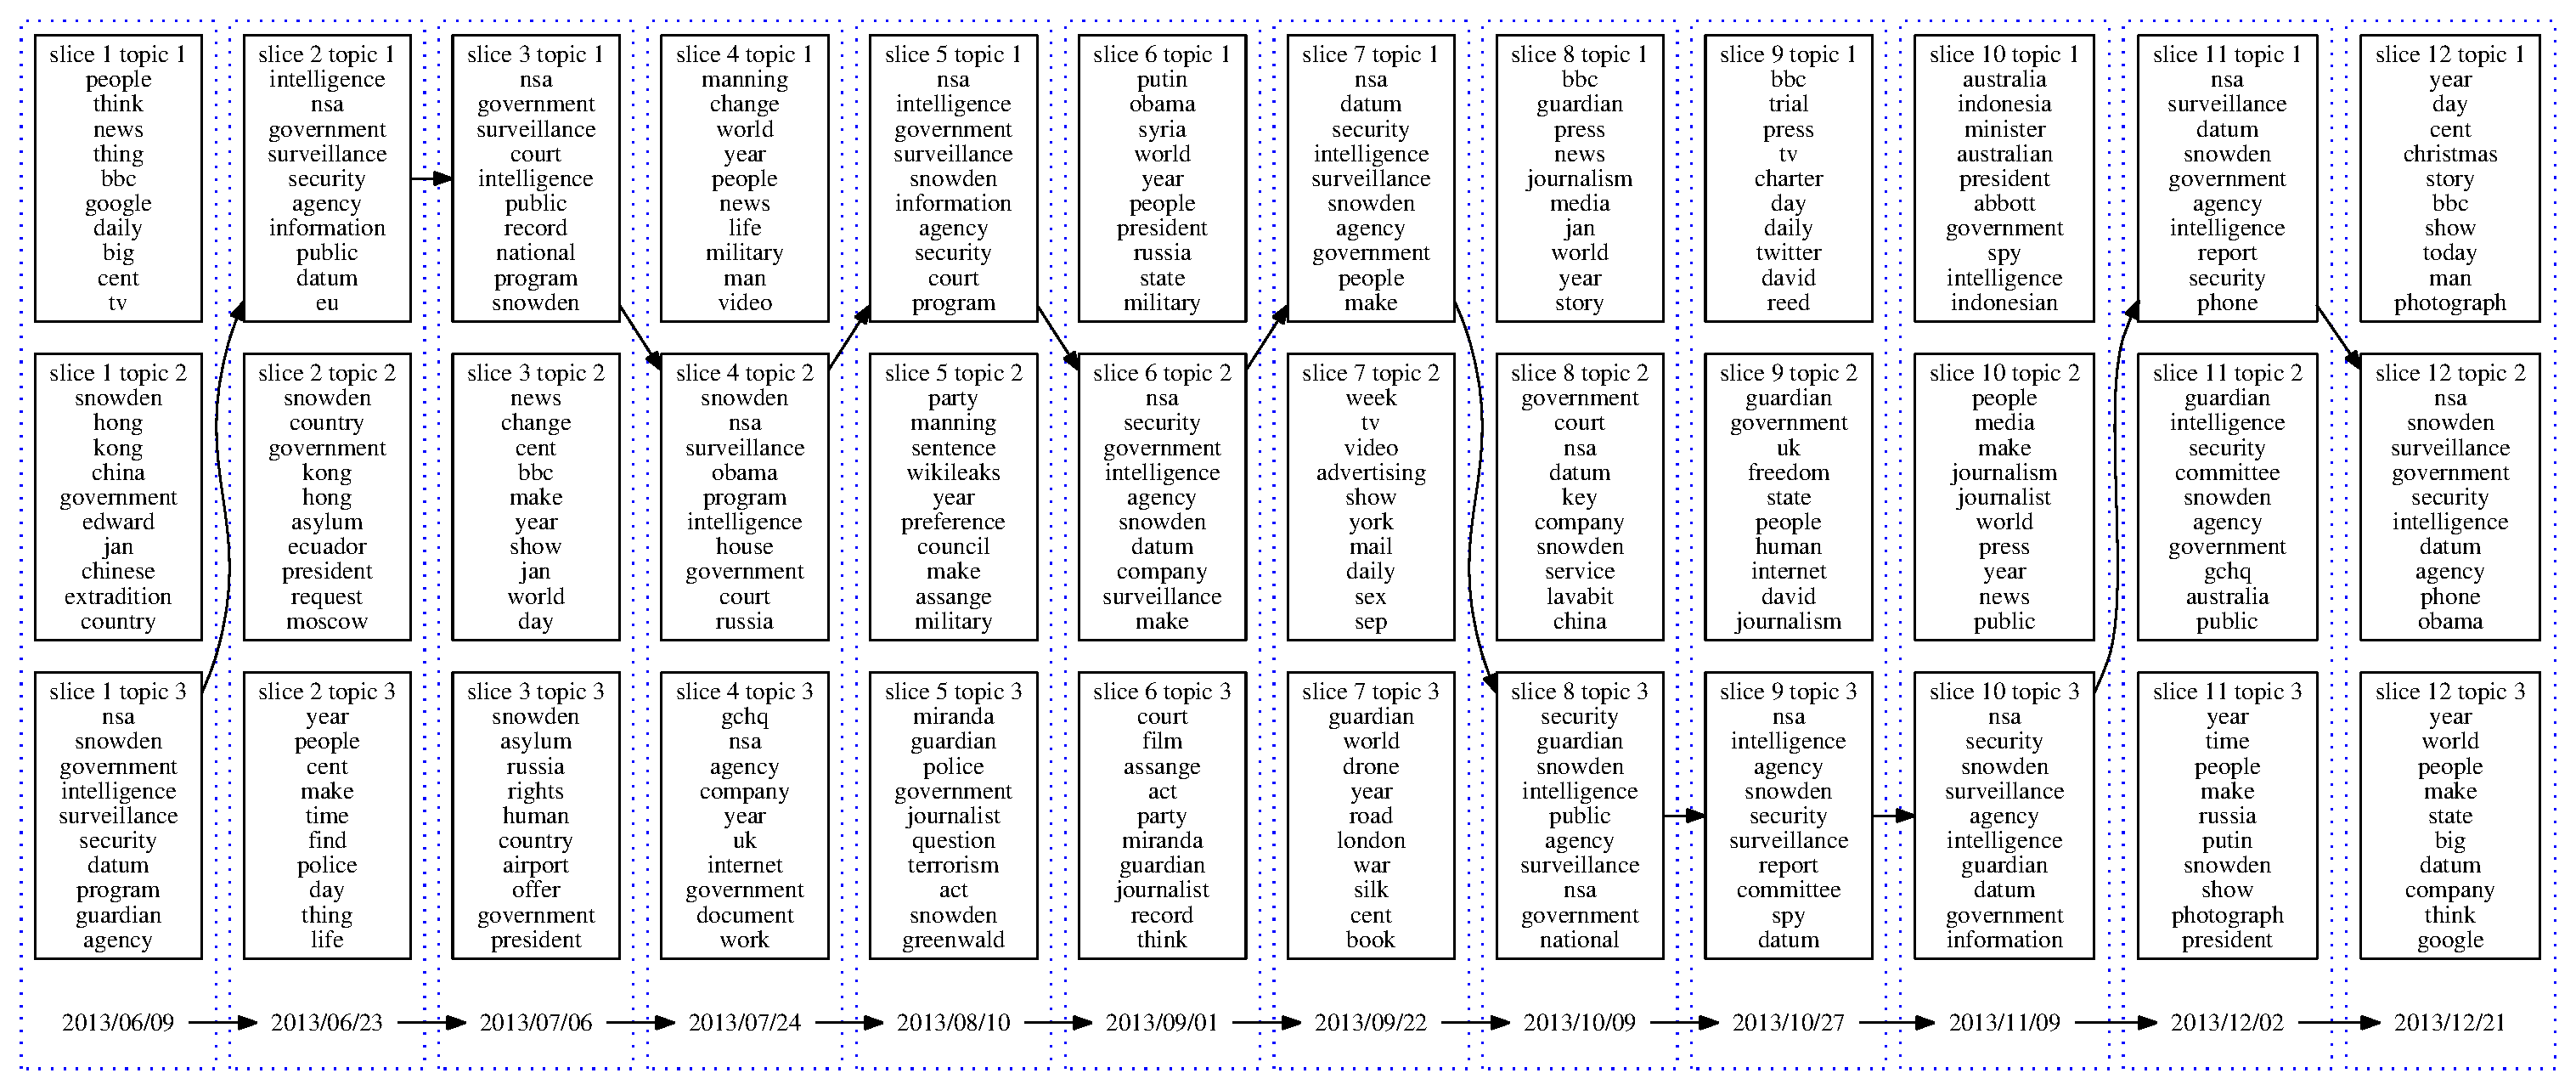
\includegraphics[width=1.0\textwidth]{evolution_lda_kmeans}
	\caption{采用本文方法获得的 "Edward Snowden" 事件的主题演化图}
	\label{fig:evolution-our}
\end{figure}
% END == 采用本文方法获得的主题演化图

通过 图 \ref{fig:evolution-our},我们可以很明了的看到,这个语料库讲的是“Edward Snowden”事件,主主题很好了反应了这一点。然后通过各个阶段的辅助主题,我们进一步分析事件的发展。从第一个阶段的辅助主题中的关键词“China, Hong Kong, TV”,我们可以知道 Snowden 是在中国香港的电视台发布了美国政府的监控计划;通过第二个阶段的辅助主题的关键词“asylum, moscow, request”,我们可以了解到 Snowden 开始向俄罗斯申请政治庇护。通过后续各个阶段的辅助主题,我们便能够对整个事件有一个全局的了解。

% BEGIN == 采用本文方法获得的主题演化图
\begin{figure}[htb]
	\centering
	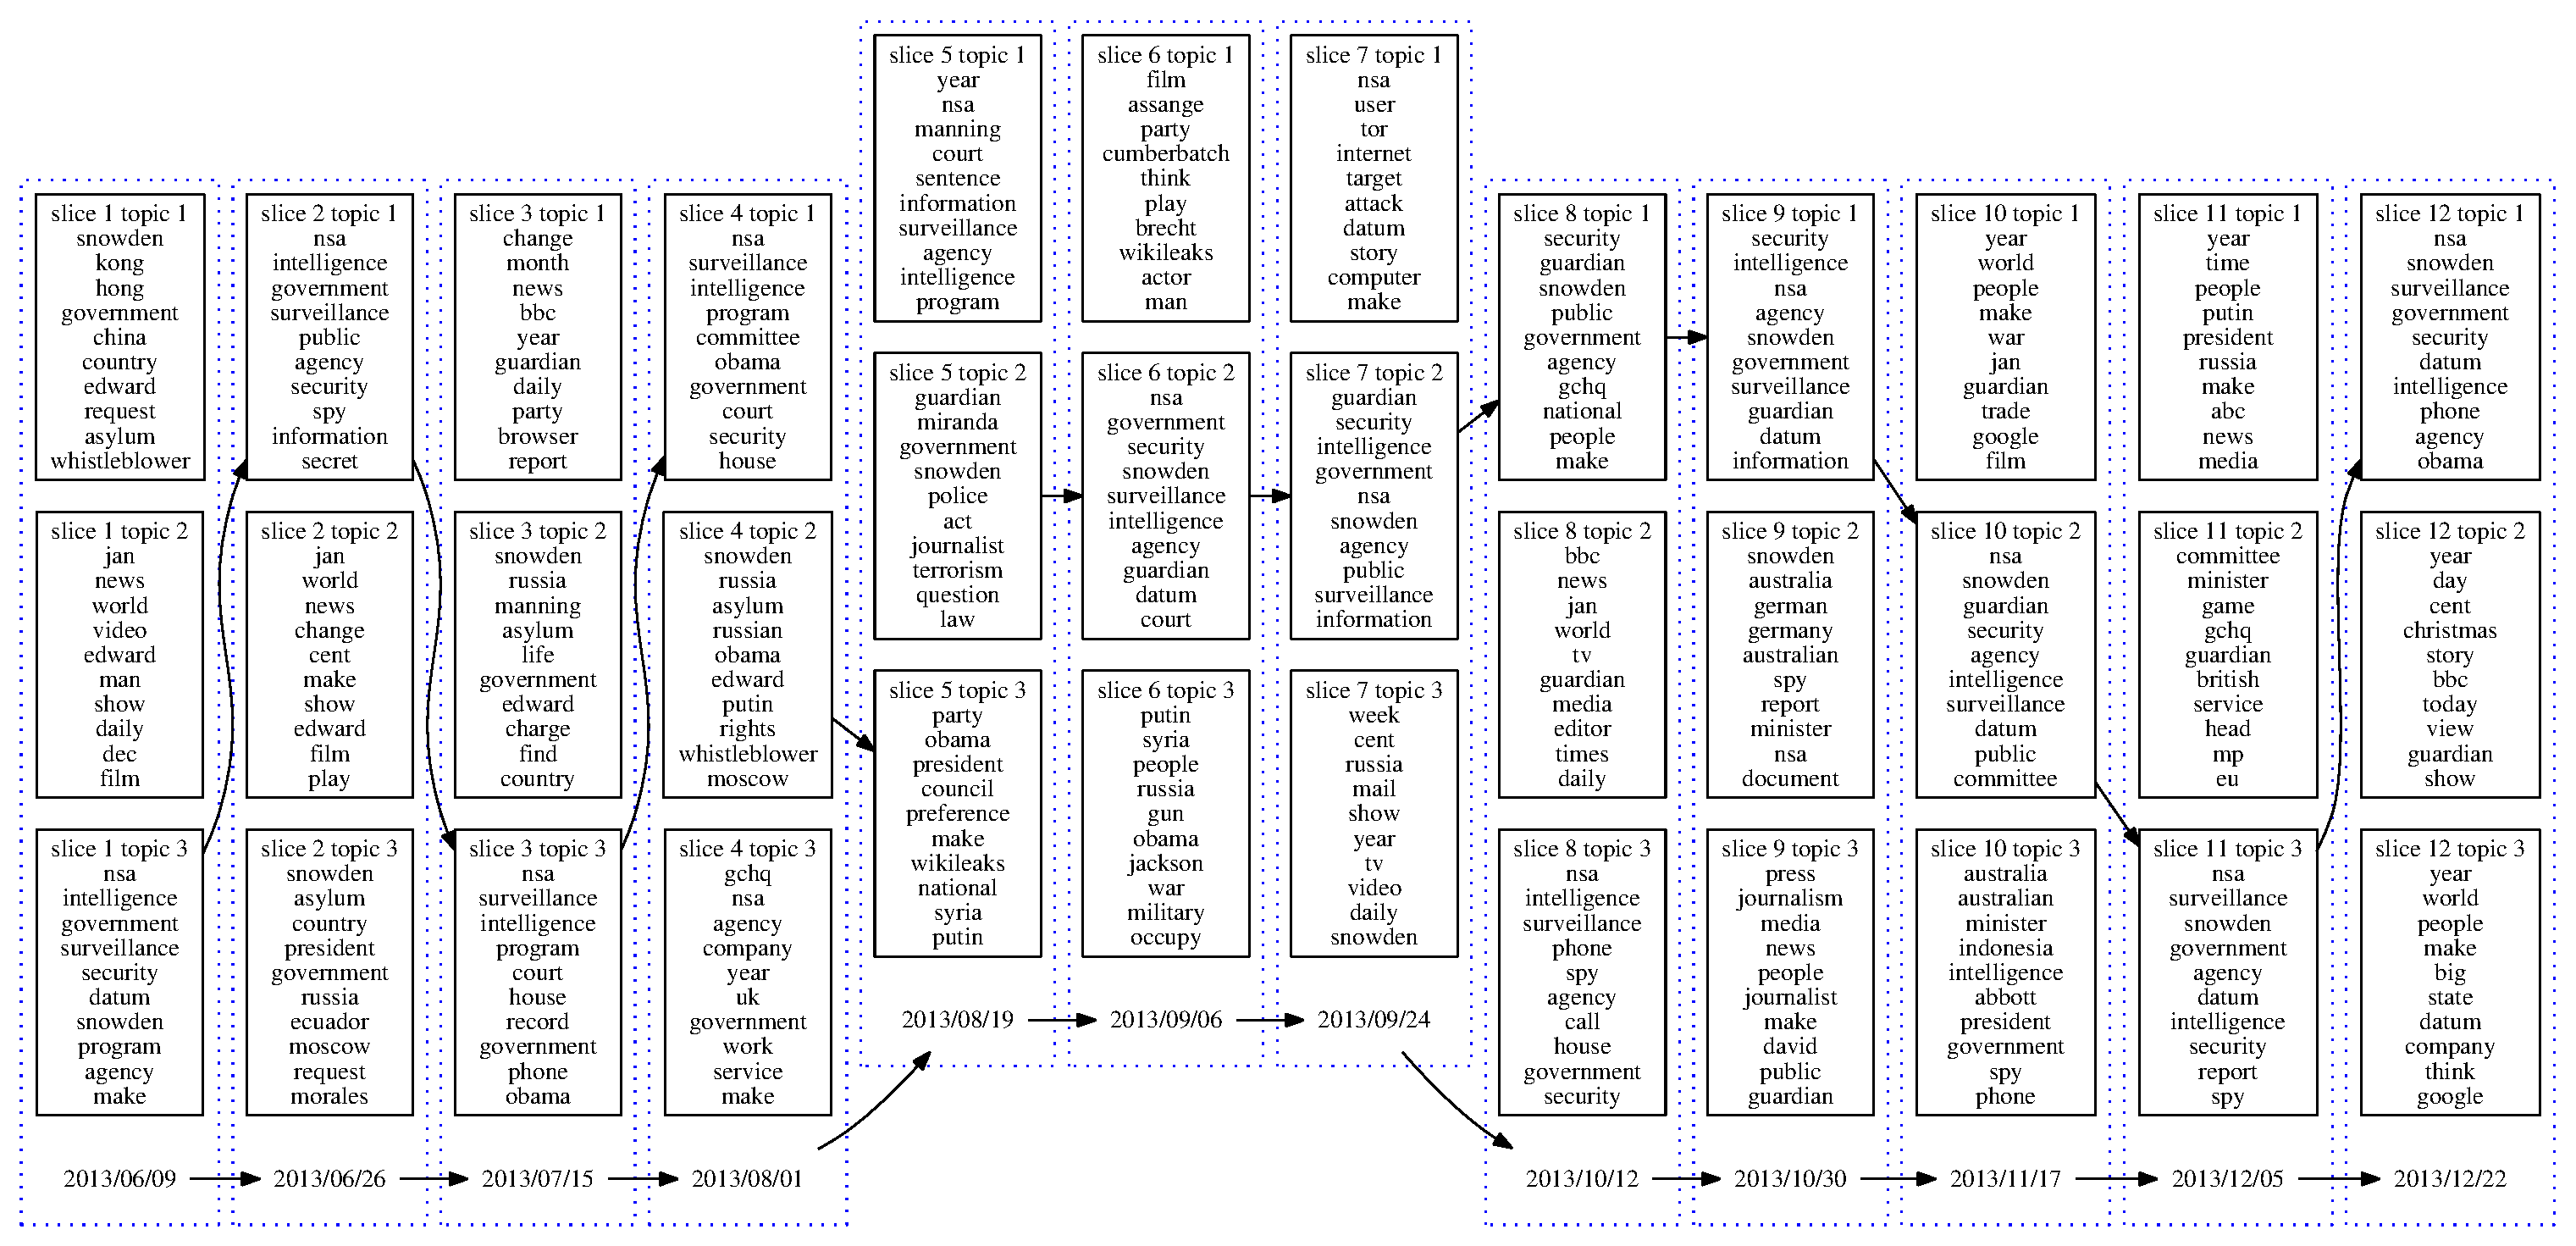
\includegraphics[width=1.0\textwidth]{evolution_lda_even}
	\caption{采用按时间均匀划分语料库的方法获得的 "Edward Snowden" 事件的主题演化图}
	\label{fig:evolution-even}
\end{figure}
% END == 采用本文方法获得的主题演化图
% BEGIN == 采用DTM获得的主题演化图
\begin{figure}[htb]
	\centering
	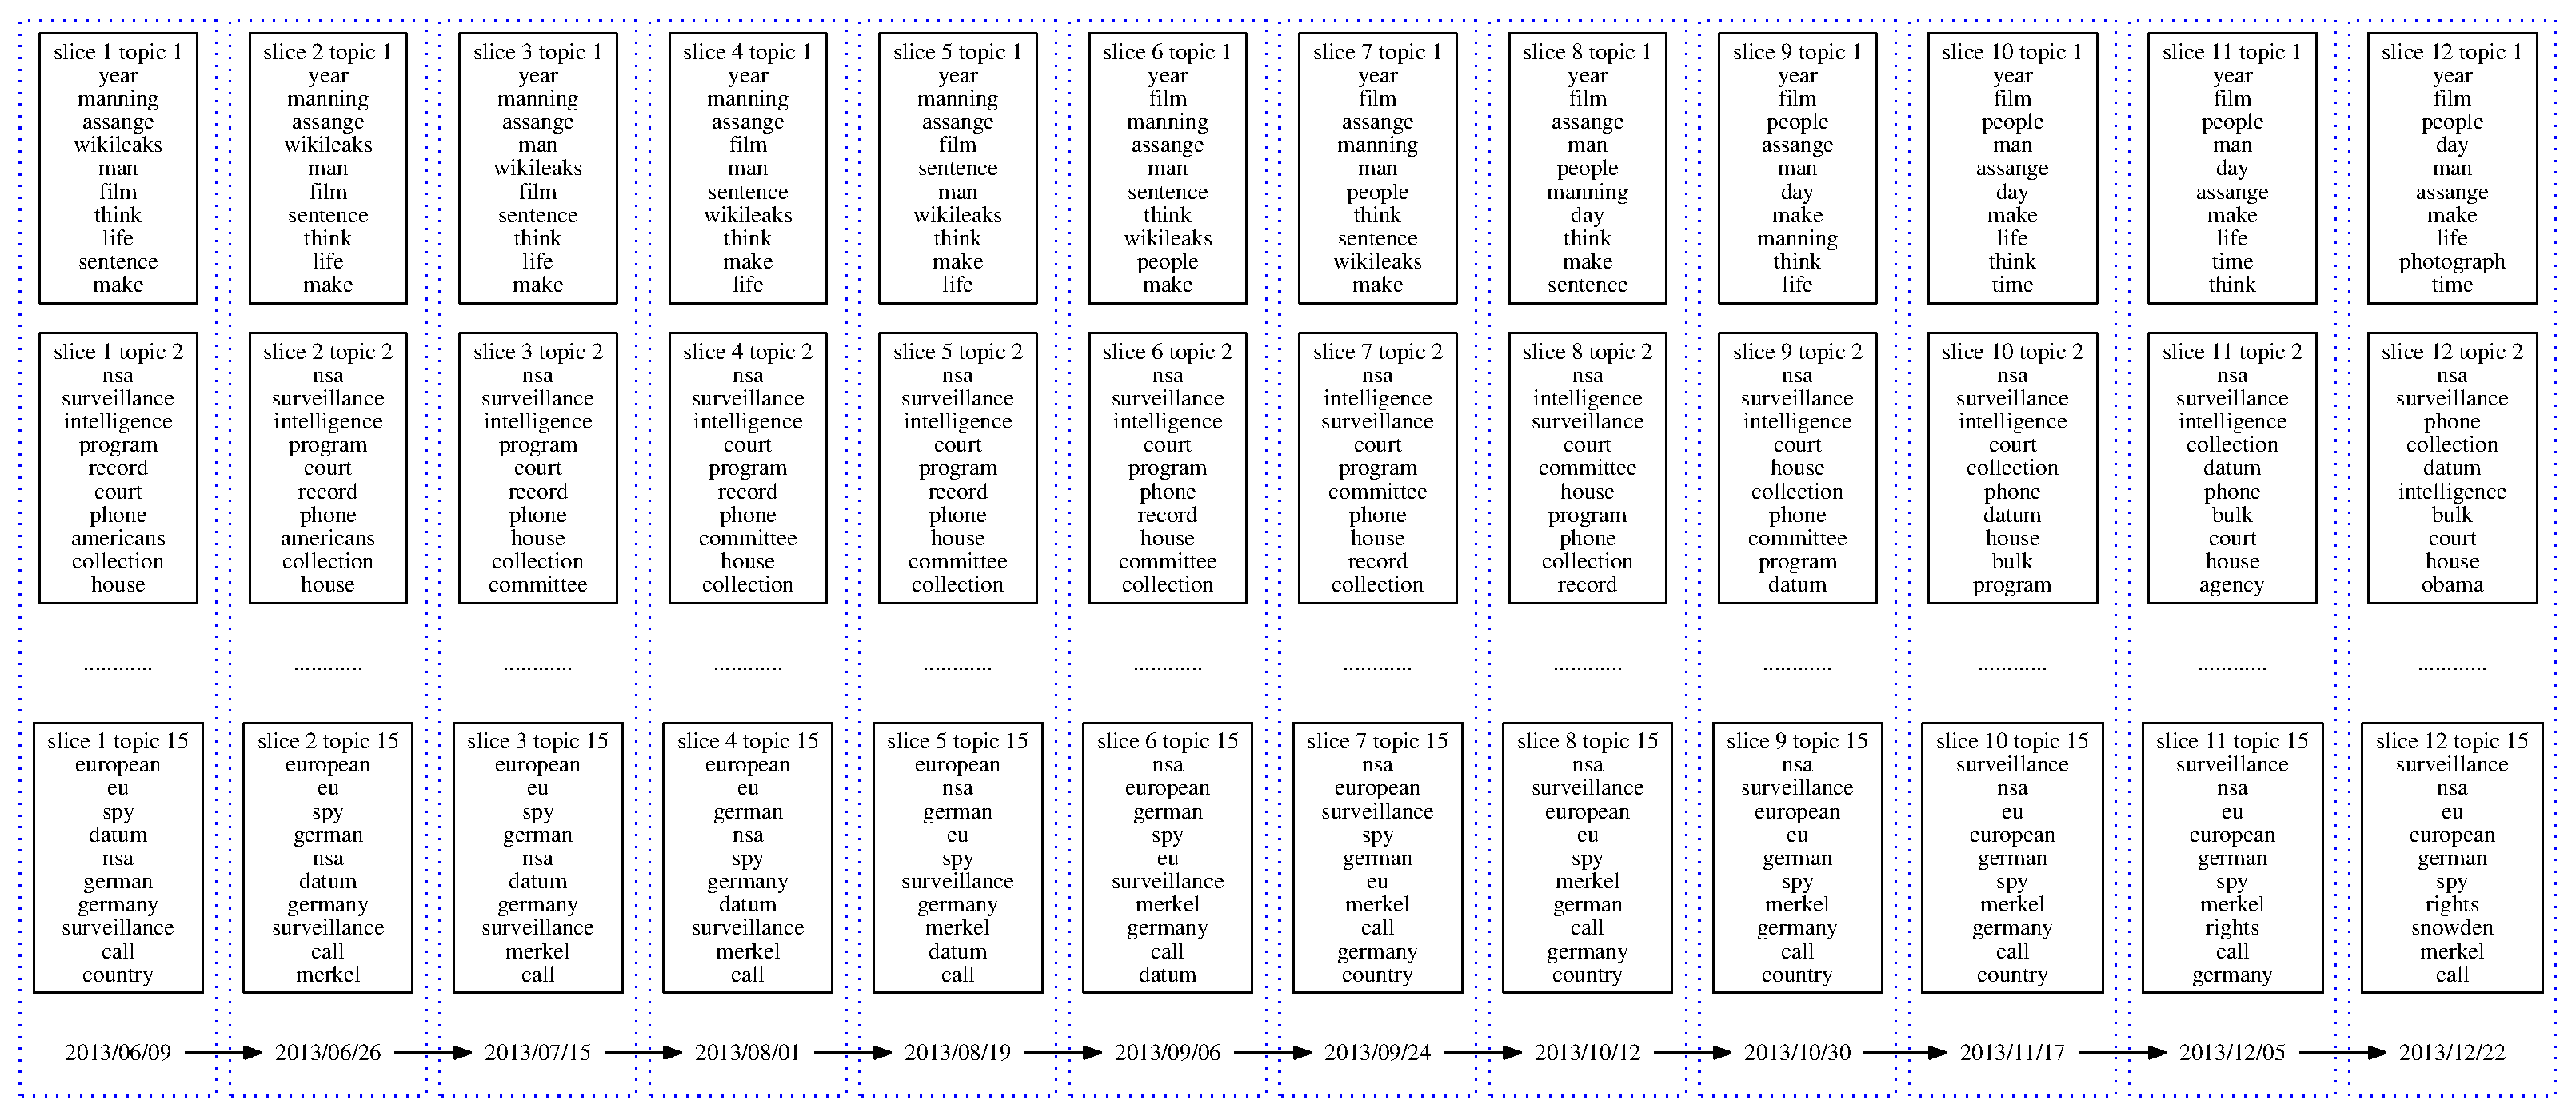
\includegraphics[width=1.0\textwidth]{evolution_dtm_15}
	\caption{采用DTM模型获得的 "Edward Snowden" 事件的主题演化图}
	\label{fig:evolution-dtm}
\end{figure}
% END == 采用DTM获得的主题演化图
在针对特定事件的语料库时,DTM表现的非常不理想,是因为DTM假设在整个语料库中主题的数目是固定的,并且所有的主题都是通过第一个时间区间演化而来的,因此它不能发现后续时间区间内新产生的主题。对于大规模的语料库,如由不同研究方法不同学科的所有学术文章构成的语料库,并且这里面包含的研究方向和方法从一开始便出现了,一直延续和发展到现在,DTM 模型能够很好的跟踪每个学科和方向随时间变化的发展。但是对于针对特定事件或特定研究领域的语料库,DTM 模型存在着先天的不足。

\subsection{文本一致性分析}
从 \ref{sec:evolution-map} 小节,我们已经看到使用本文提出的方法在抽取某一事件的主题演化图时有明显的优势。本小节我们将通过实验数据说明为什么会产生这样的结果,同时验证本章最初提出的假设 \ref{hyp:coherence} 。
\label{sec:coherence-result}
% BEGIN == 文档一致性分析图
\begin{figure}[htb]
	\centering
	\subfloat[$TCR_5$]{
		\includegraphics[width=0.5\textwidth]{cover_rate_snowden_5_topic}
		\label{fig:tcr_5}}
	\subfloat[Average $TCR_n$]{
		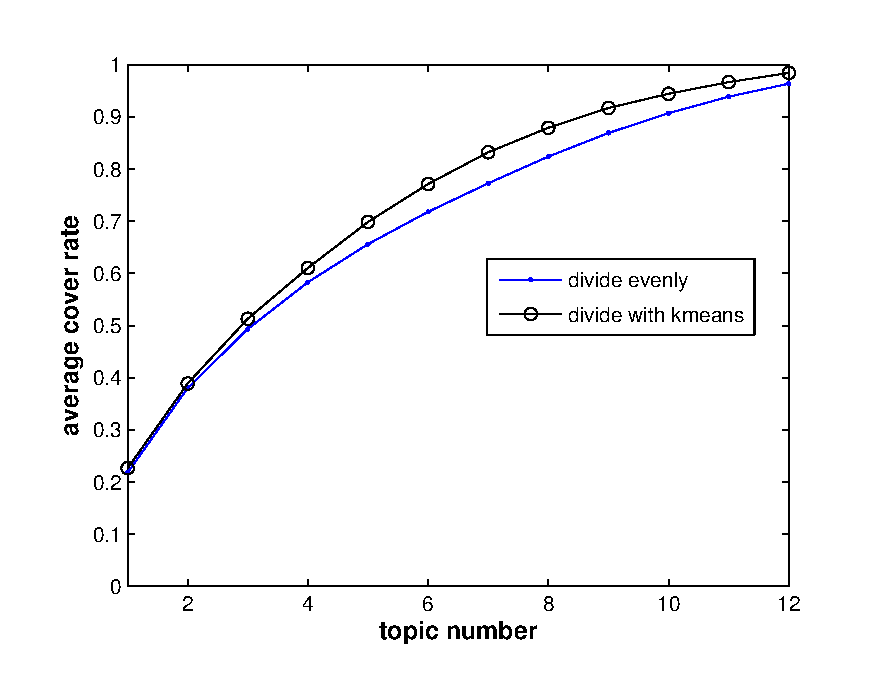
\includegraphics[width=0.5\textwidth]{avg_cover_rate_snowden}
		\label{fig:tcr_n}}	
	\caption{“Edward Snowden” 语料库的 $TCR_n$ 分析}
	\label{fig:tcr}
\end{figure}
% END == 文档一致性分析图

图 \ref{fig:tcr} 展示的是我们通过两种不同的方法对“Edward Snowden”事件相关的语料库进行划分后,得到的子语料库内文本一致性数据。蓝色线条实星点表示的折线代表的是我们按时间均匀划分语料库得到的数据,黑色线空心点表示的折线是采用本文提出的 Algorithm \ref{algo:ada-kmeans} 进行语料库划分得到的结果。图 \ref{fig:tcr_5} 表示的是概率最大的前5个主题在不同时间段内的文档覆盖率,从图中可以看到,采用本文方法在大部分的时间段内,文本一致都要高于均匀划分。为了更好的衡量前n个主题在所有时间段内的平均文档覆盖率,我们分别计算了前1个到前12个主题,在所有时间段内的平均文档覆盖率。从 图 \ref{fig:tcr_n} 采用本文方法进行划分所得的子语料库中文本一致性普遍高于均匀划分。结合 \ref{sec:evolution-map} 小节的实验结果和 图 \ref{fig:tcr} 的数据,我们可以认为本文最初提出的假设 \ref{hyp:coherence}是正确的。 

\section{本章小结}
本小节我们首先分析了针对新闻事件的报道的时序分布情况,并针对这一分布特点提出了一个简单有效的语料库划分算法 adaptive k-means algrithm。采用我们提出的划分算法所得到的子语料库能够很好的保证文档的一致性,而我们认为一致性越高的文档集合更加有利于我们使用主题模型进行信息挖掘,通过我们的实验结果也验证了这一假设。接着我们提出了一套用于跟踪新闻事件主题演化的分析框架,基于该框架我们最终能将新闻事件自动的划分为几个阶段,并且发现每个阶段内事件的最新动向和发展,同时通过主主题很好的衔接各个的阶段。

本章提出的方法着眼于挖掘针对某一个事件或某一研究领域的特定语料库,通过利用它们在时序分布上的信息,结合主题模型进行深度挖掘,试图获得它们更加丰富的主题演化信息。这一出发点有别于其他一些研究者,专注于规模大且主题比较混合的语料库。本文提出的方法也可以很好的与其它一些文本分析的方法进行结合,如自动摘要抽取等。将来我们希望能将本方法进一步完善,并开发一套可以供用户交互的新闻事件分析程序,以便让媒体人或普通的读者能够在更短的时间内更好的了解事件的整体发展。




